\documentclass{beamer}

\usefonttheme{professionalfonts} % using non standard fonts for beamer
\usefonttheme{serif} % default family is serif

\usepackage{hyperref}
%\usepackage{minted}
\usepackage{animate}
\usepackage{graphicx}
\def\Put(#1,#2)#3{\leavevmode\makebox(0,0){\put(#1,#2){#3}}}
\usepackage{colortbl}
\usepackage{tikz}
\usepackage{amssymb}
\usepackage{enumerate}
\usepackage{arydshln}
\usepackage{algorithm}
\usepackage{algpseudocode}

\colorlet{lightred}{red!25}
\colorlet{lightgreen}{green!25}
\beamertemplatenavigationsymbolsempty

\newcommand\blfootnote[1]{%
  \begingroup
  \renewcommand\thefootnote{}\footnote{#1}%
  \addtocounter{footnote}{-1}%
  \endgroup
}

\makeatletter

%% Textclass specific LaTeX commands.
\newcommand\makebeamertitle{\frame{\maketitle}}%
\AtBeginDocument{%
  \let\origtableofcontents=\tableofcontents
  \def\tableofcontents{\@ifnextchar[{\origtableofcontents}{\gobbletableofcontents}}
  \def\gobbletableofcontents#1{\origtableofcontents}
}
%% User specified LaTeX commands.
\usetheme{Malmoe}
\useoutertheme{infolines}
\addtobeamertemplate{headline}{}{\vskip2pt}
\setbeamercovered{transparent}

\makeatother

%%%%%%%%%%%%%%%%%%%%%%%%%%%%%%%%%%%%%%
%% Main document
%%%%%%%%%%%%%%%%%%%%%%%%%%%%%%%%%%%%%%
\begin{document}
\title[PFLOCK report]{PFLOCK Report}
\author[AC]{Andres Calderon}
\institute[Spring'20]{University of California, Riverside}
\makebeamertitle
\newif\iflattersubsect

\AtBeginSection[] {
    \begin{frame}<beamer>
    \frametitle{Outline} 
    \tableofcontents[currentsection]  
    \end{frame}
    \lattersubsectfalse
}

\AtBeginSubsection[] {
    \begin{frame}<beamer>
    \frametitle{Outline} 
    \tableofcontents[currentsubsection]  
    \end{frame}
}

\begin{frame}{Task ID and Core/Thread mapping}
  \begin{itemize}
  \item Technically a mapping between taskId and core/thread is not possible\footnote{\tiny More info at \url{https://tinyurl.com/ycjvxtne}}...
    \begin{itemize}
    \item Apache Spark will run a Task as a Runnable process managed by the JVM.
    \item JVM interacts directly with the OS to deal with those processes.
    \item There is no guarantee an OS process run in only one core.
    \end{itemize}
  \item However, based on the lifetime of a Task (launchTime and finishTime) we can explore how concurrent are the Tasks...
  \end{itemize}
\end{frame}

\begin{frame}{Task histogram}{Task distribution\footnote{\tiny click to enlarge...}}
  \centering
  \href{https://www.cs.ucr.edu/~acald013/public/Research/Figures/TasksHist17.pdf}{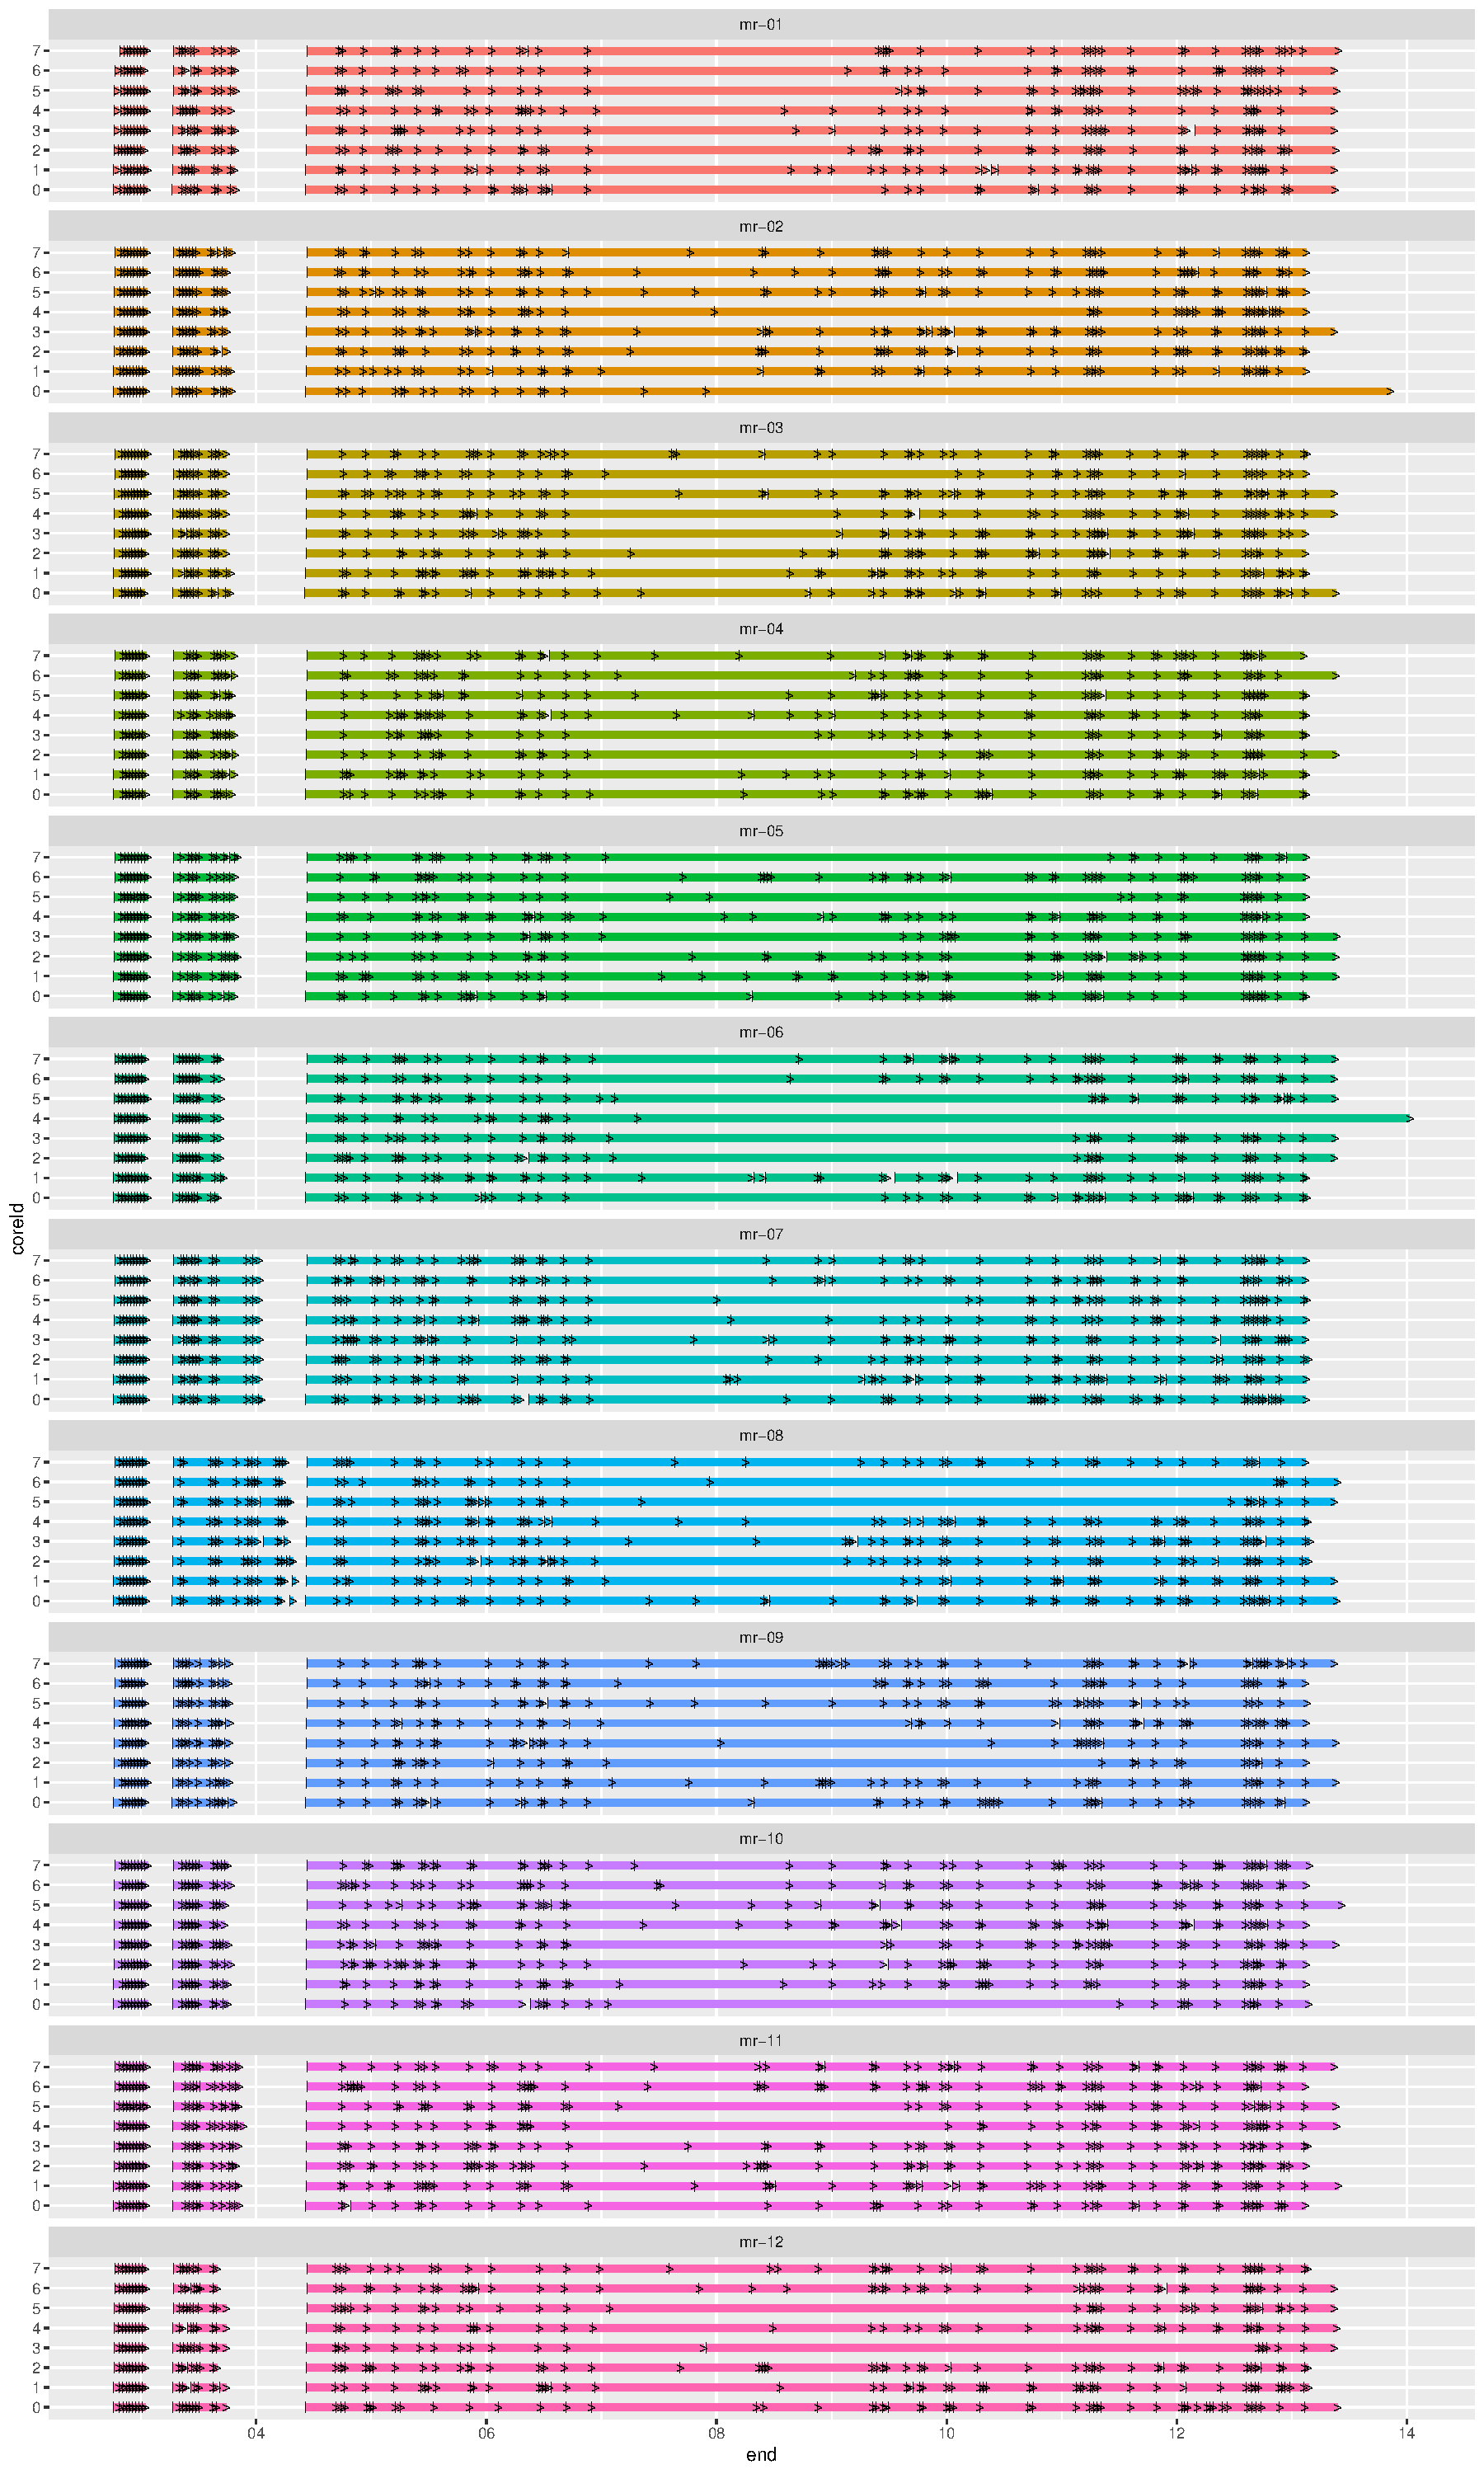
\includegraphics[scale=0.125]{figures/TasksHist17}}
\end{frame}

\begin{frame}{Node usage}
    \centering
    \begin{tabular}{l l}
        \hline
                        & n \\ \hline
        Min.         & 1.00\\  
        1st Qu.    & 8.00 \\ 
        Median    & 8.00\\  
        Mean       & 7.95 \\ 
        3rd Qu.    & 8.00 \\
        Max.        &13.00  \\ \hline
    \end{tabular} \\
    \vspace{0.5cm}
    \begin{tabular}{c c c c c c c c c c c c c}
    1 & 2 & 3 & 4 & 5 & 6 & 7 & \textbf{8} & 9 & 10 & 11 & 12 & 13\\ 
   310 & 315 & 489 & 788 & 374 & 697 & 198 & \textbf{121763} & 4721 & 616 & 77 & 11 & 2 \\ 
    \end{tabular}
\end{frame}

\begin{frame}{Task histogram}{Top 10 tasks by duration}
  \centering
  \href{https://www.cs.ucr.edu/~acald013/public/Research/Figures/TopTaskHist.pdf}{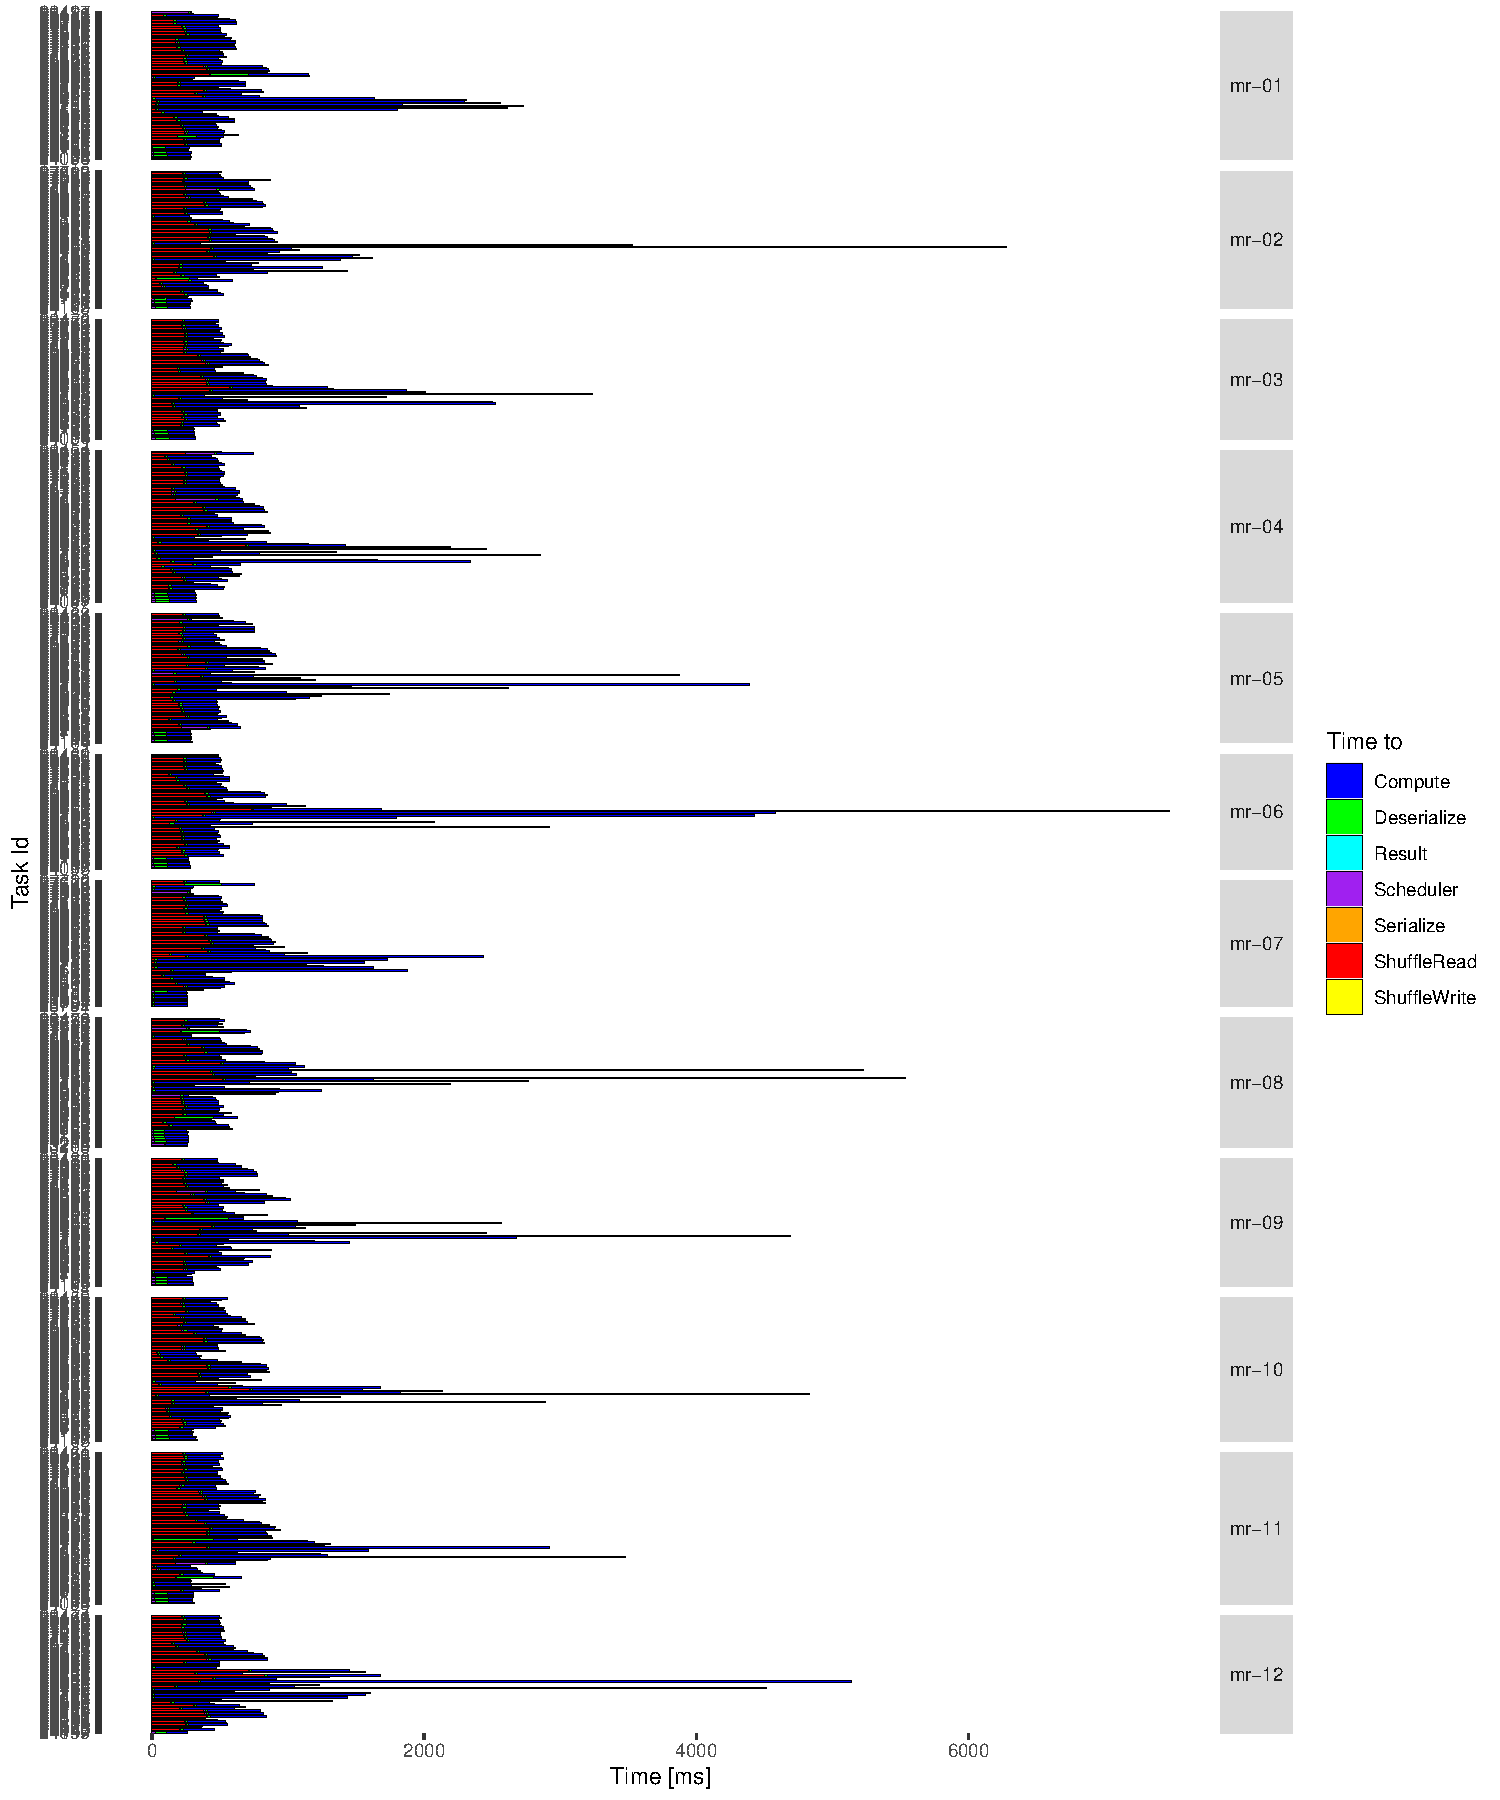
\includegraphics[scale=0.25]{figures/TopTasksHist_pflock17}}
\end{frame}

\begin{frame}{Task-Data Mapping}
    \begin{itemize}
        \item Class \texttt{TaskContext} allows to collect information about the task execution on runtime.
        \item Methods \texttt{partitionId()} and \texttt{taskAttemptId()} give us the ID of the RDD partition and the task it was assigned.
    \end{itemize}
    
\end{frame}

\begin{frame}{Task-Data Mapping}
  \centering
  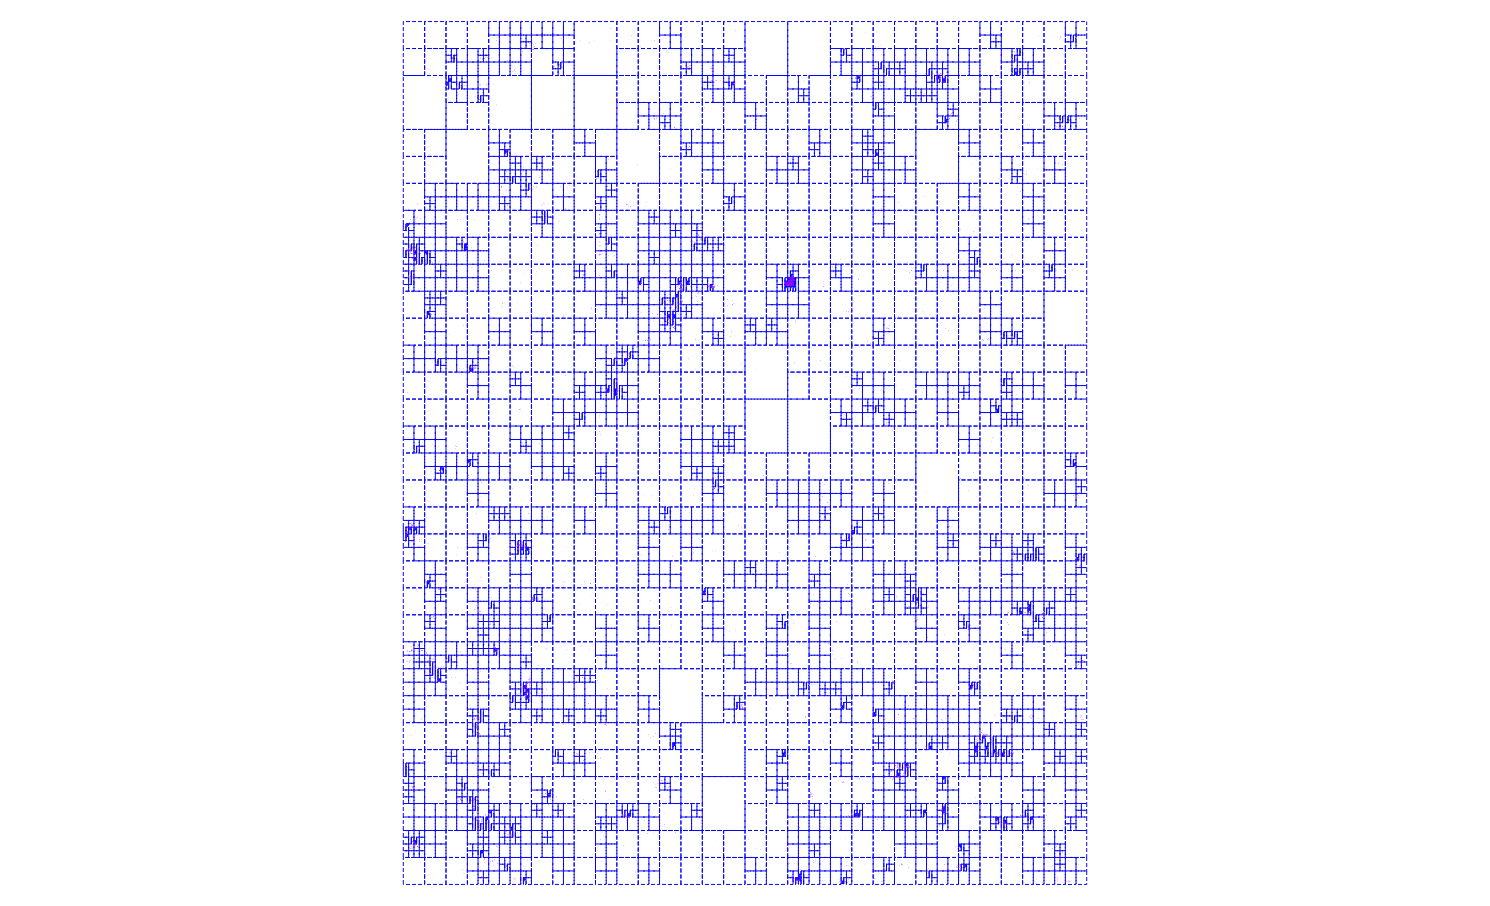
\includegraphics[width=\textwidth]{figures/BadPartitions3}
\end{frame}
\begin{frame}{Task-Data Mapping}
  \centering
  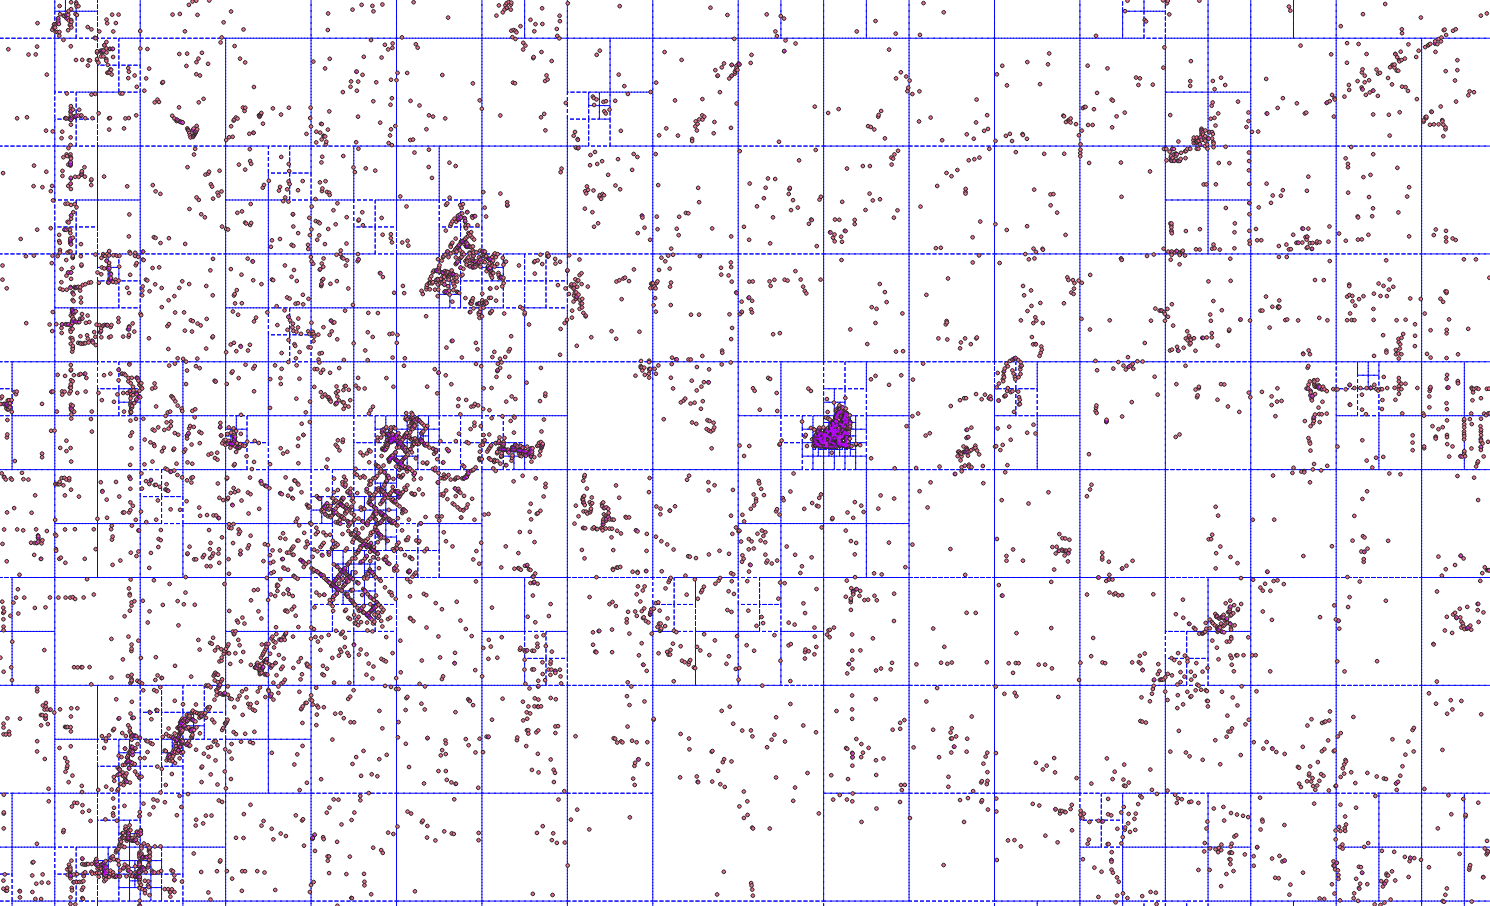
\includegraphics[width=\textwidth]{figures/BadPartitions2}
\end{frame}
\begin{frame}{Task-Data Mapping}
  \centering
  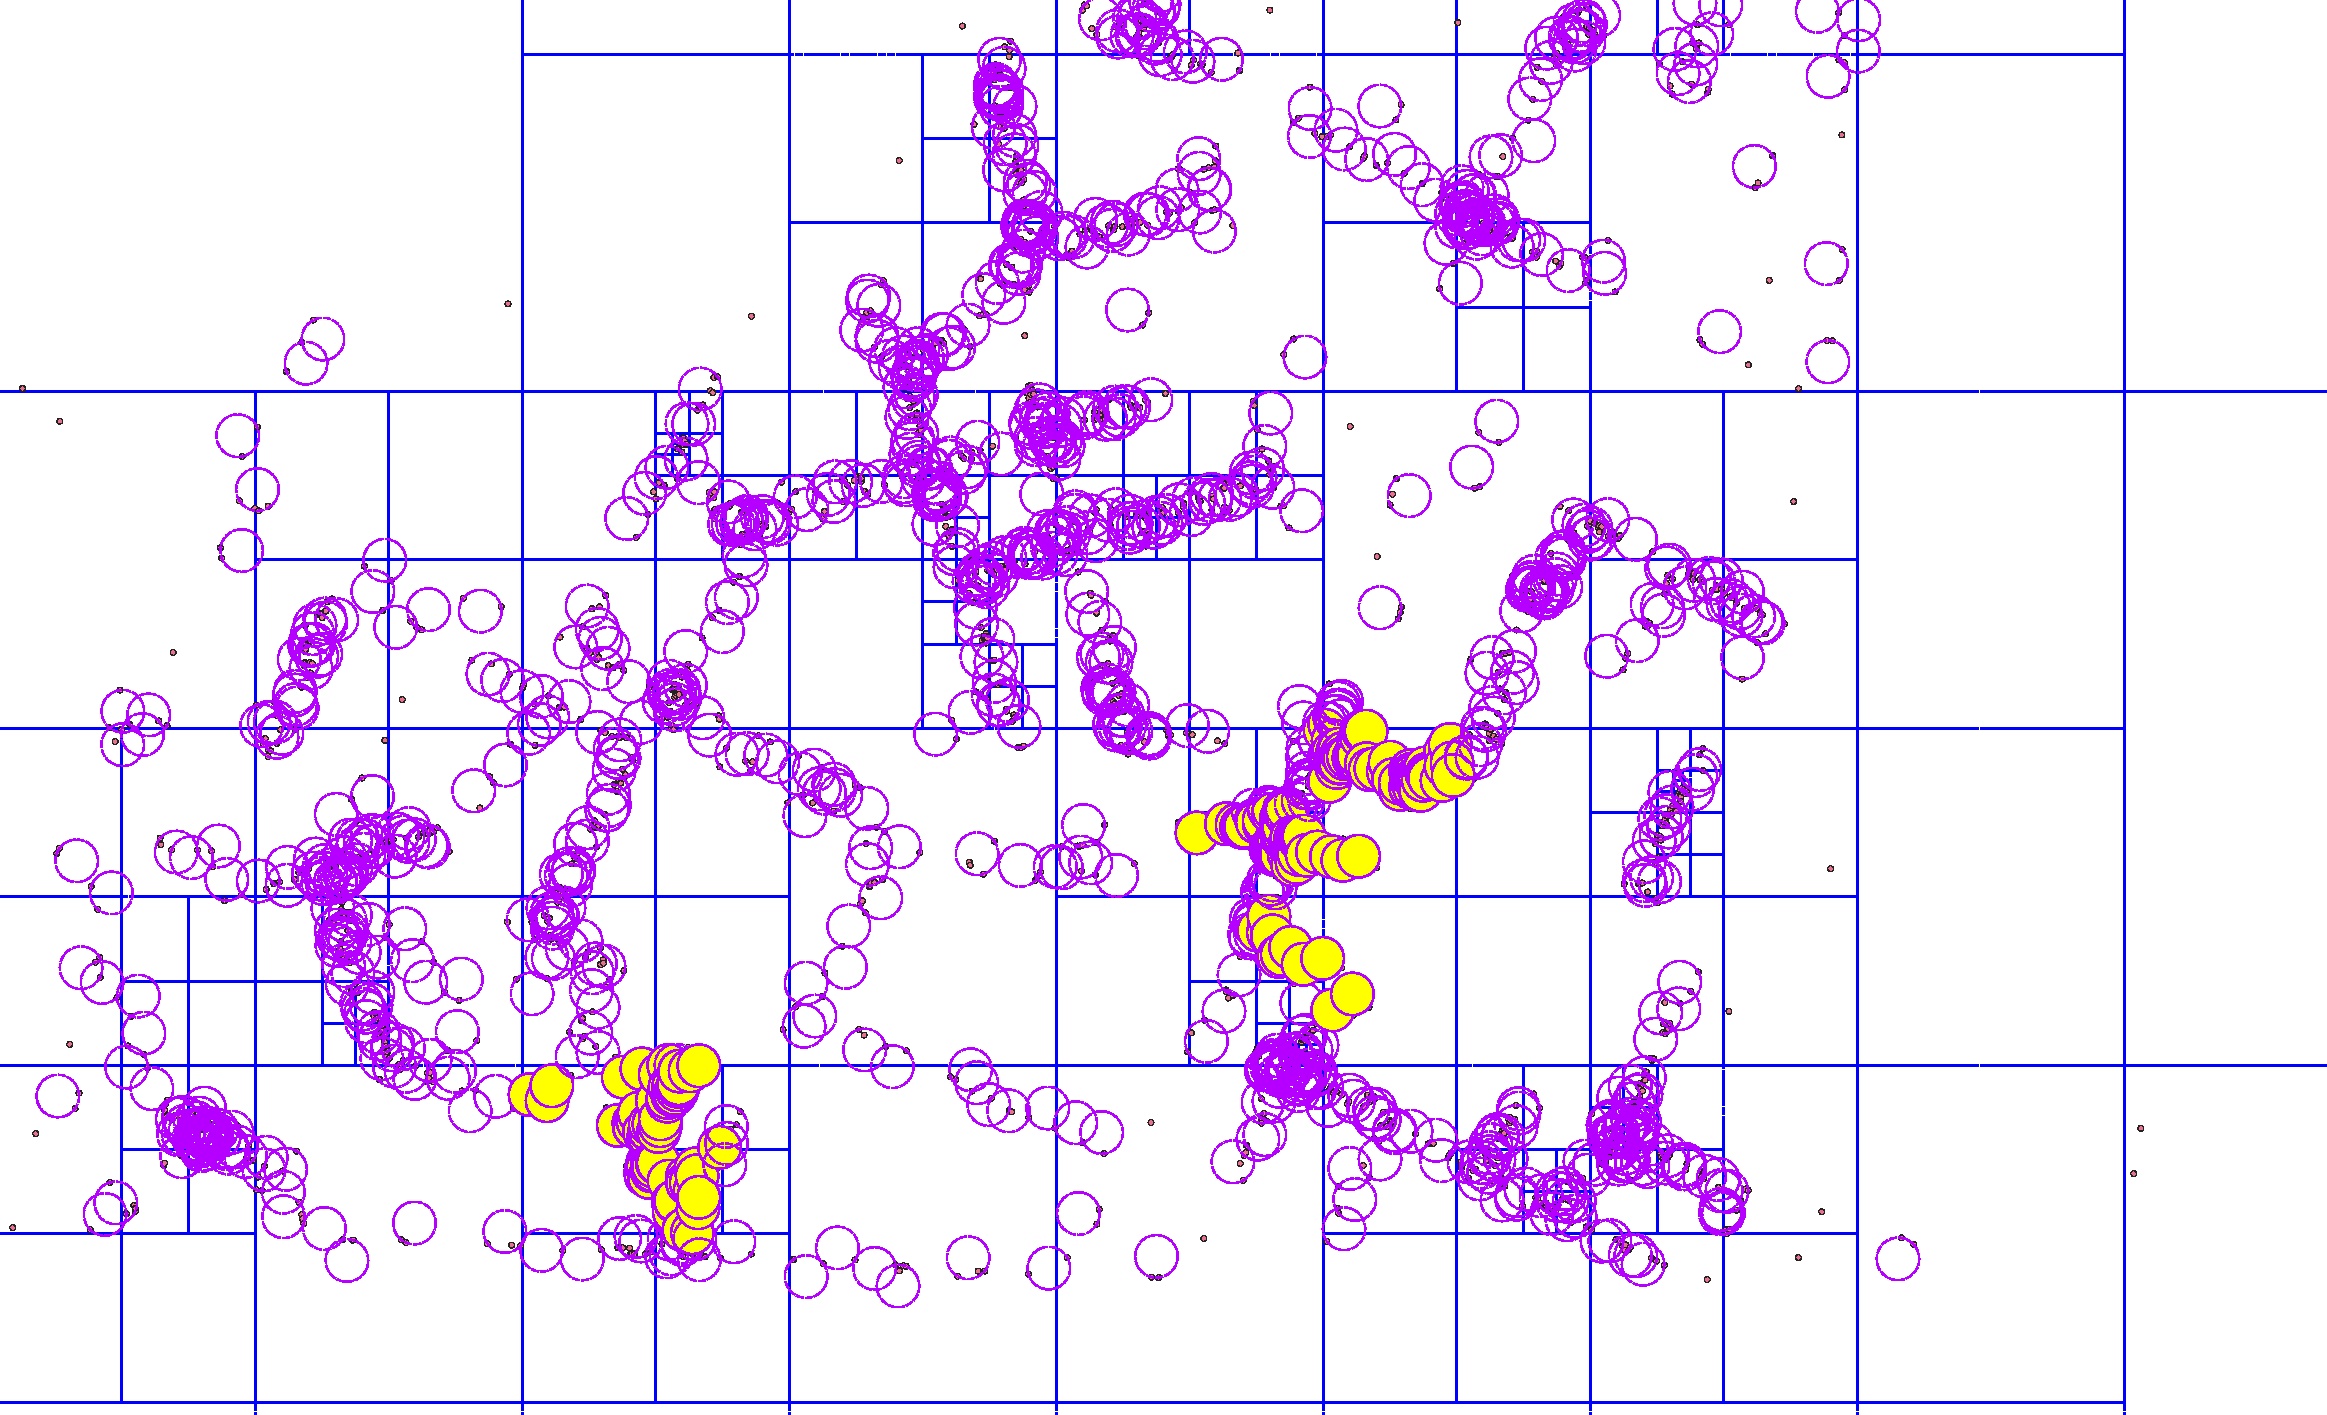
\includegraphics[width=\textwidth]{figures/BadPartitions}
\end{frame}

\begin{frame}{What's next}
    \begin{itemize}
        \item Measure the impact of very small partitions.
        \item Still dealing with shuffle cost.
        \item Give a try with a different dataset.
    \end{itemize}
\end{frame}

\end{document}

